\documentclass{report}
\usepackage{graphicx}
\usepackage{ctex}
\usepackage{hyperref}

\title{\Huge{\textbf{商业报告}}}
\author{谢品文\ $\cdot$\ 何胜威\ $\cdot$\ 洪皓倬\ $\cdot$\ 邓世辕}

\begin{document}
\maketitle

\tableofcontents

\newpage

\section*{1. 摘要}
\addcontentsline{toc}{chapter}{1. 摘要}

此份报告是由谢品文、何胜威、洪浩卓、邓世辕四人共同完成的。报告中将会对\textbf{托马斯微积分}这本致命的微积分教材进行介绍,包括对该产品的介绍、市场分析、营销策略等。

\section*{2. 产品介绍}
\addcontentsline{toc}{chapter}{2. 产品介绍}

\subsection*{2.1 产品概述}
\addcontentsline{toc}{section}{2.1 产品概述}

\textbf{托马斯微积分(Thomas' CALCULUS)}是一本微积分教材的经典,被广泛用于世界各地大学的微积分教学,由美国麻省理工大学数学家乔治·托马斯(George B. Thomas, Jr.)编写,于1951年首次出版。该书的第十五版于2022年出版,由Joel R. Hass(加利福尼亚大学戴维斯分校)、Christopher E. Heil(乔治亚理工学院)、Maurice D. Weir(美国海军研究生院)和Przemyslaw Bogacki(欧道明大学)编写。

50多年来,该书平均每4至5年就有一个新版面世(最新第十五版),每版较之先前版本都有不少改进之处,体现了这是一部锐意革新的教材;与此同时,该书的一些基本特色始终注意保持且有所增强,说明它又是一部重视继承传统的教材。与现行中文高等数学教材相比,其基本内容和结构框架有着许多近似之处,但在题材选取和处理上又有更多不同特色,尤其是,突出应用和数学建模,重视数值计算和程序应用。在适时引进现代数学和新学科知识等方面,更有不少精彩之处。

\subsection*{2.2 产品特点}
\addcontentsline{toc}{section}{2.2 产品特点}

\noindent\textbf{图文并茂、全彩印刷}

\noindent 该书的每一页都是彩色印刷,采用优质滑面纸张,且配有大量的插图,使得学生在阅读时能够更加直观地理解复杂的数学概念。
~\\

\noindent\textbf{内容严谨、层次分明}

\noindent 该书延续了先前版本的优点,内容清楚分明了正式及非正式的探讨,并指出了他们之间的区别。书中每一章节从相对浅白易懂、非正式的讨论开始,然后逐步深入,直至给出严格的定义和定理。这种方法使得学生能够在不失严谨性的前提下,更加容易地理解微积分的概念。
~\\

\noindent\textbf{由浅入深、循序渐进}

\noindent 该书的从最基础的函数概念开始,逐步引入极限、导数、积分等概念,直到后来的多元微积分,内容章节规划合理,难度由浅入深,循序渐进,只要学生按照书中的章节顺序学习,就能够很好地掌握微积分的知识。
~\\

\noindent\textbf{大量习题、题型多样}

\noindent 该书的每一章都有大量的习题,题型多样,让学生能够在学习完每一章的内容之后,通过大量的练习,巩固所学的知识。
~\\

\noindent\textbf{注重应用、强调实践}

\noindent 除了大量的计算题,让学生能够更加熟练地掌握微积分的计算方法之外,该书的每一章的习题中都有跨越各领域的应用题,这些题目涉及到了物理、化学、工程、经济、生物、医学、社会科学等领域,使得学生能够更加直观地理解微积分的应用。
~\\

\noindent\textbf{善用科技、简化计算}

\noindent 该书在部分习题中,引导学生使用科技手段,如计算机、计算机代数系统(CAS)、数值计算软件等,简化计算过程,使得学生能够更加专注于微积分的应用,而不是被繁琐的计算所困扰。
~\\

\noindent\textbf{奇数题解、方便查阅}

\noindent 该书末尾附有奇数题的解答,方便学生查阅,检验自己的答案是否正确。此外,该书还额外出版了完整的解答手册,方便教师查阅。

\newpage
\subsection*{2.3 目录架构}

本书共分为19章,涵盖了大学微积分I、II、III的全部内容,具体内容如下:

\begin{enumerate}
    \item 函数(微积分I)
    \item 极限与连续(微积分I)
    \item 导数(微积分I)
    \item 导数应用(微积分I)
    \item 积分(微积分I)
    \item 定积分应用(微积分I)
    \item 超越函数(微积分I)
    \item 积分方法(微积分II)
    \item 一阶微分方程(微积分II)
    \item 无限数列与级数(微积分II)
    \item 参数方程与极坐标(微积分II)
    \item 空间解析几何与向量(微积分III)
    \item 向量函数与空间运动(微积分III)
    \item 偏导数(微积分III)
    \item 多元积分(微积分III)
    \item 积分与向量场(微积分III)
    \item 二阶微分方程(微积分III)
    \item 复数
    \item 周期函数
\end{enumerate}

\newpage

\subsection*{2.4 产品内容}
~\\
\noindent\textbf{课文内容}
\begin{center}
    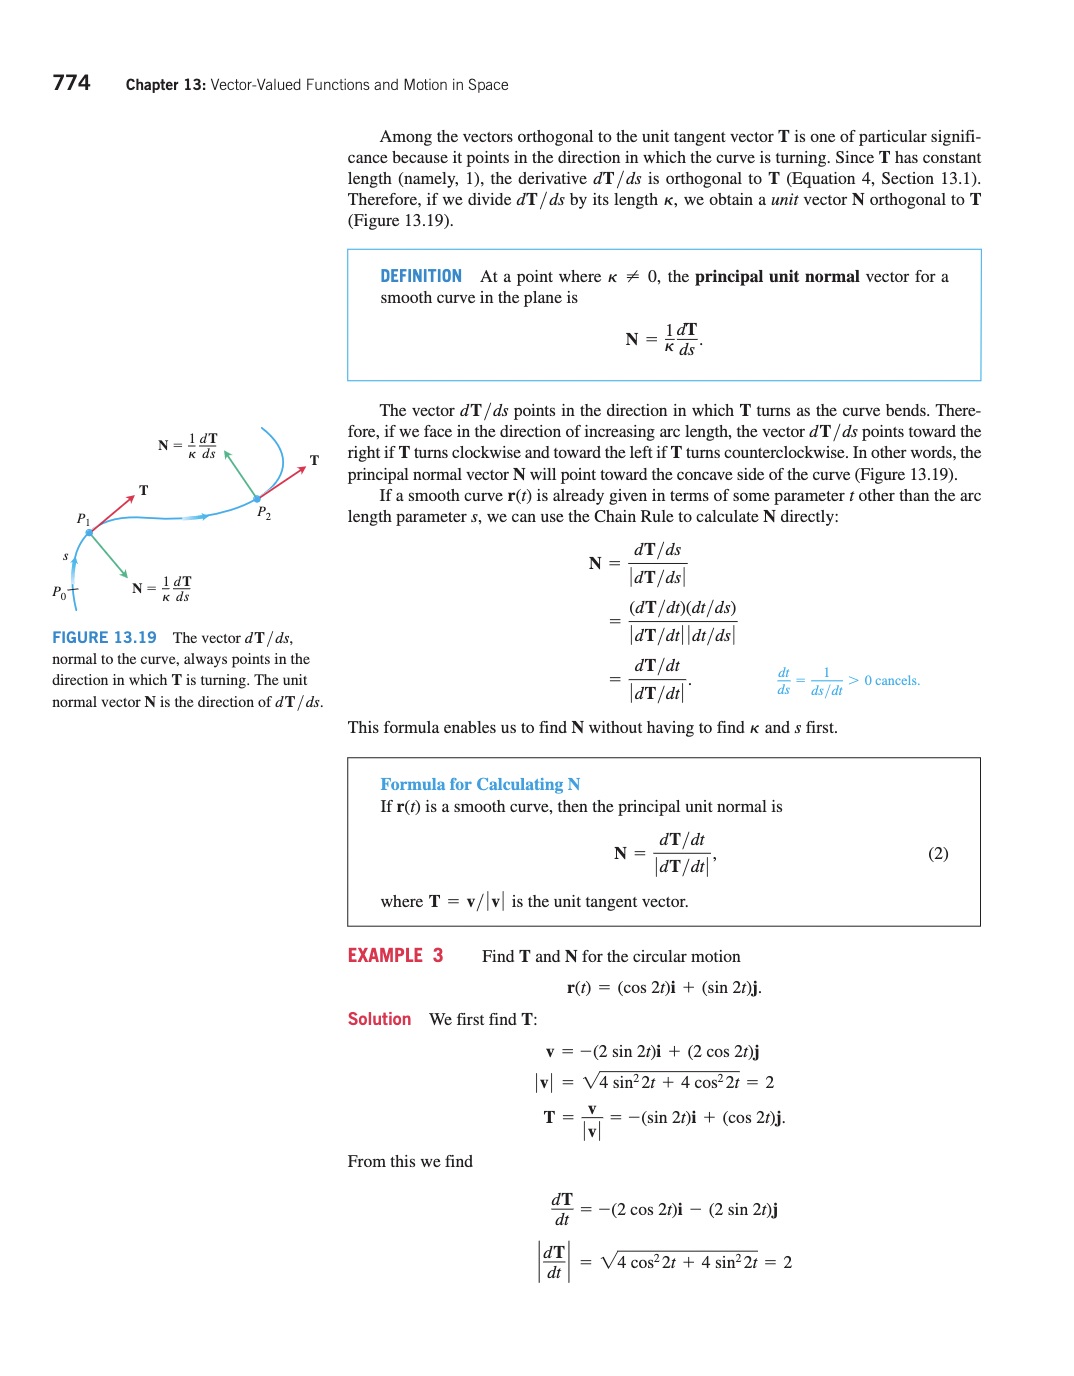
\includegraphics[width=\textwidth]{./content1.png}
\end{center}
\newpage
\noindent\textbf{章节习题}
\begin{center}
    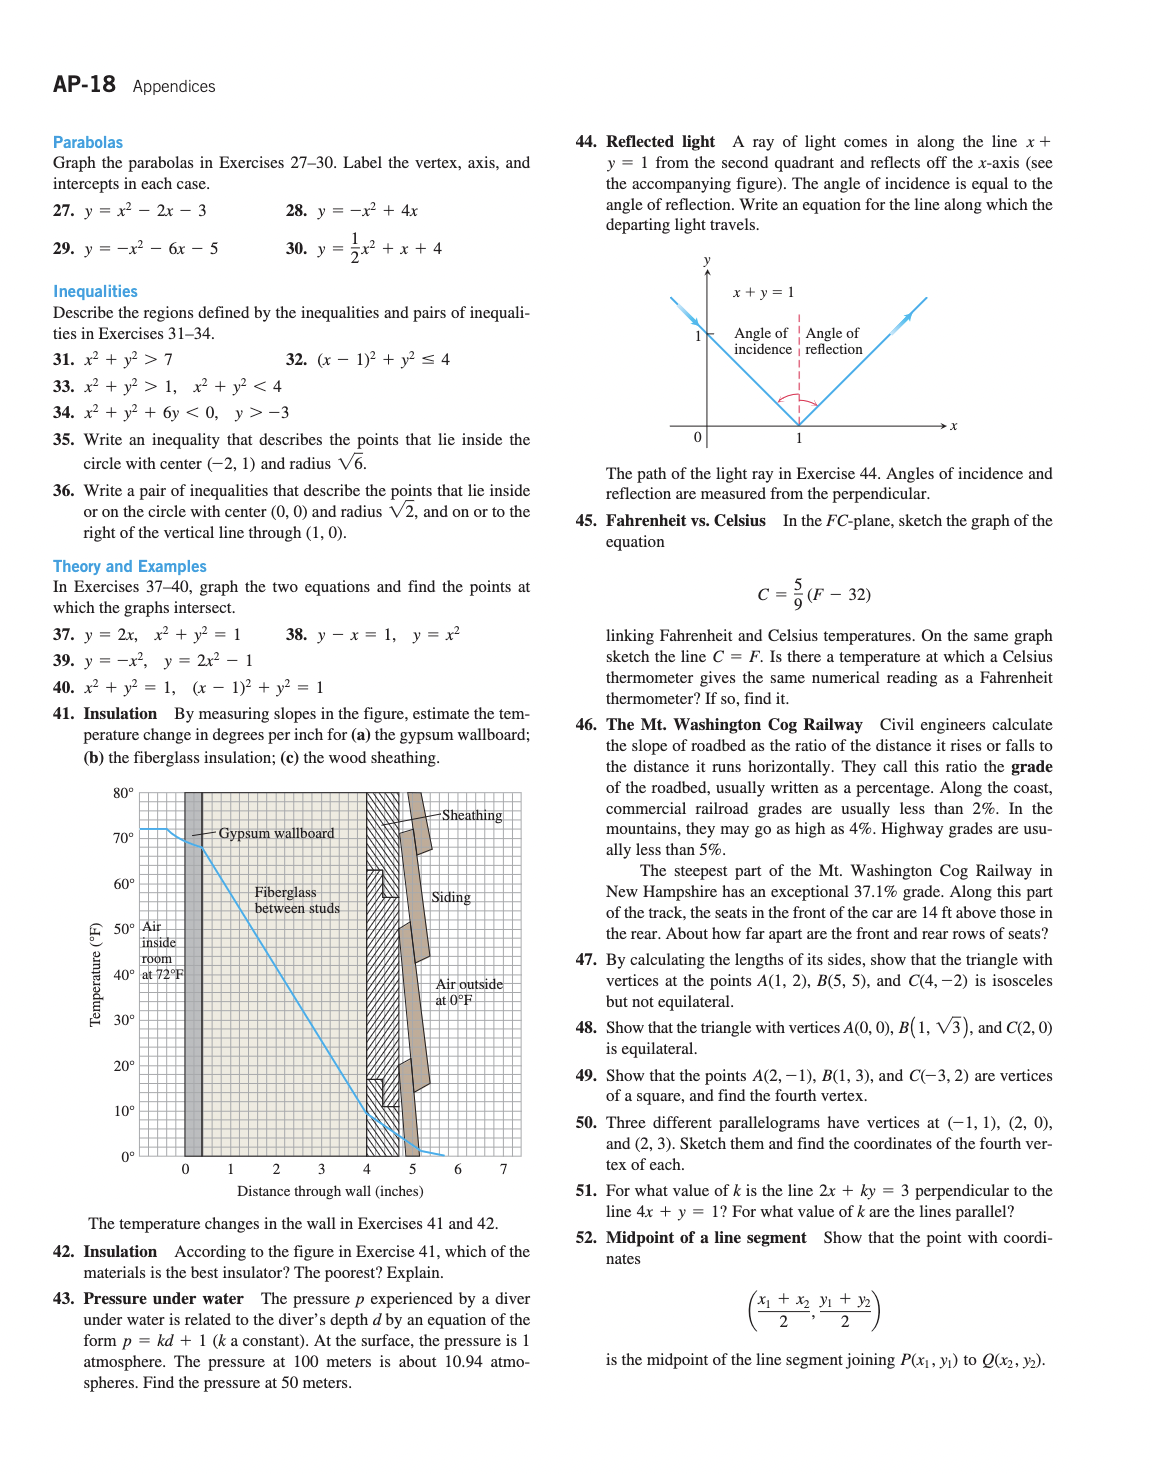
\includegraphics[width=\textwidth]{./content2.png}
\end{center}
\newpage
\noindent\textbf{奇数题解答}
\begin{center}
    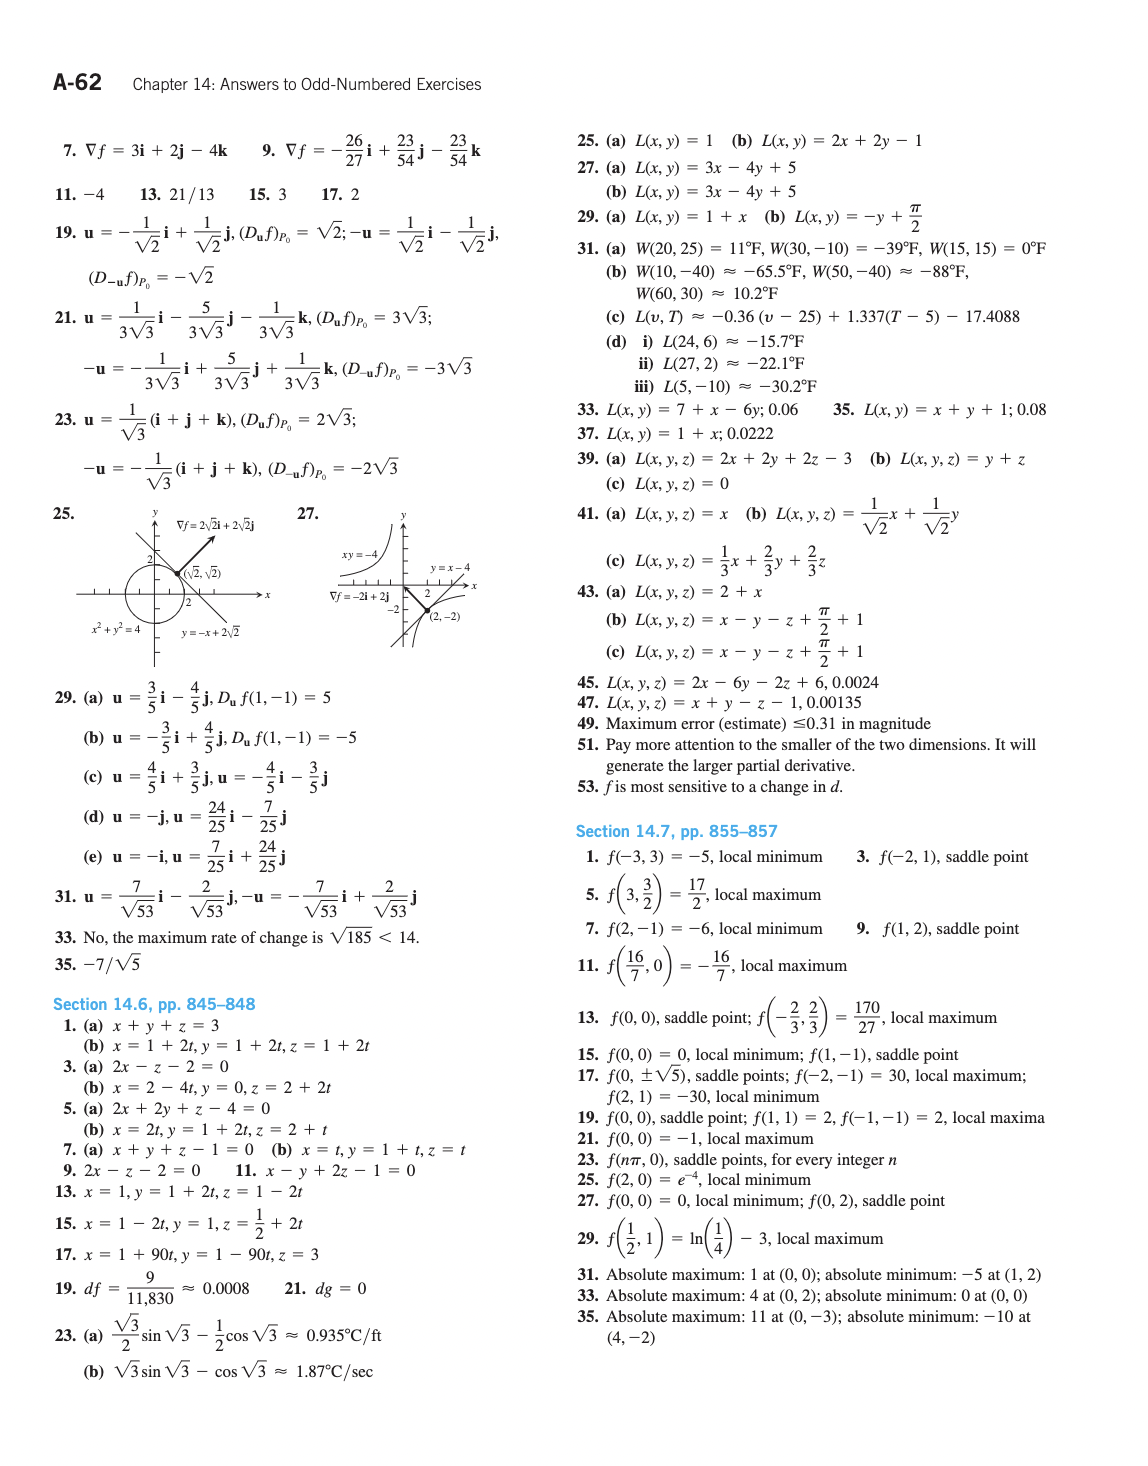
\includegraphics[width=\textwidth]{./content3.png}
\end{center}

\newpage

\section*{3. 市场分析}
\addcontentsline{toc}{chapter}{3. 市场分析}

\subsection*{3.1 市场概述}
\addcontentsline{toc}{section}{3.1 市场概述}

数学教材市场在高等教育和自助学习领域中扮演着关键角色。这个市场涵盖了不同领域教材,从代数、三角函数等基础数学概念到复分析、场论、拓扑学等高级数学领域,每一本书都有其适用于不同教育水平和专业领域。微积分是数学领域中的基石,在绝大多数大学的许多科系中,微积分都是必修课,因此微积分教材的质量对学生和教育机构至关重要。

\subsection*{3.2 市场区隔}
\addcontentsline{toc}{section}{3.2 市场区隔}

\noindent\textbf{多种语言}

\noindent 此书是一本备受全球高校和学院欢迎的微积分教材,涵盖了微积分的广泛内容。它的市场份额在许多国家和地区都很大。此外,它还被翻译成多种语言,以满足不同国家和地区的语言需求。
~\\

\noindent\textbf{不同格式}

\noindent 托马斯微积分提供了许多在线资源,以满足不同学习需求。此外,除了价格相对昂贵的实体书,它还提供了价格更低的电子书版本。
~\\

\noindent{\textbf{学生及专业人士需求}}

\noindent 每年都有大量学生及工程师、经济学家等专业人士需要学习微积分,而Thomas' Calculus以其清晰的教学方法和多样的学习资源,吸引了广泛的学生用户群。

\subsection*{3.3 目标市场}

\noindent\textbf{大学和学院}

\noindent 此书主要针对大学和学院的微积分课程。它适用于不同学科领域的学生,包括数学、工程、自然科学、计算机科学和商科等。
~\\

\noindent\textbf{本科生和研究生}

\noindent 此书适用于本科和研究生水平的学生,包括那些学习微积分的新手和那些正在深入研究微积分的高级学生。
~\\

\noindent\textbf{专业人士}

\noindent 此书也适用于专业人士,如工程师、科学家、经济学家和金融学家等,他们需要微积分的知识来解决实际问题。
~\\

\noindent\textbf{全球市场}

\noindent 此书在全球范围内具有市场,适用于不同国家和地区的教育体系。它通常提供多国语言版本,以满足不同学生的需求。
~\\

\noindent\textbf{教育机构}

\noindent 学校、学院和大学通常是此书的主要采购者,他们将这本教材作为课程的标配或建议的教材。
~\\

\noindent\textbf{不同计量单位}

\noindent 此书除了有采用帝国单位制的版本之外,还出版了采用了国际单位制(SI)的版本,以满足不同地区的学生需求。

\subsection*{3.4 市场定位}
\addcontentsline{toc}{section}{3.4 市场定位}

\noindent\textbf{高质量的微积分教材}

\noindent 此书以其深刻的数学理论和清晰的教学方法而闻名,又因其高质量彩色印刷,被定位为高质量的微积分教材。它为学生提供了深入理解微积分概念和技能的机会。
~\\

\noindent\textbf{广泛的学科覆盖}

\noindent 此书内容涵盖了不同学科领域的微积分需求,包括初级微积分、工程微积分和商业微积分等。这种多样性使其适用于各种不同的学科和专业。
~\\

\noindent\textbf{学生友好的教材}

\noindent 此书强调其易于理解的教学方法和大量的示例和练习题,以帮助学生掌握微积分的核心概念。

\newpage
\noindent\textbf{全球市场覆盖}

\noindent 被定位为一个适用于全球市场的微积分教材,被翻译成多国语言版本以满足不同地区的学生需求。

\section*{行销策略}
\addcontentsline{toc}{chapter}{4. 行销策略}

\subsection*{4.1 产品定价}
\addcontentsline{toc}{section}{4.1 产品定价}

托马斯微积分的价格在不同地区和版本之间有所不同。但是,由于此书属于高质量教育资源,因此其价格相对较高。在马来西亚,实体书的价格普遍在RM200至RM300左右,而在美国,实体书的价格普遍在\$100至左右。电子书的价格通常比实体书便宜。在出版商Pearson的官网中,可用\$10左右的价格租购电子书。

\subsection*{4.2 产品品牌}
\addcontentsline{toc}{section}{4.2 产品品牌}

托马斯微积分是一本备受欢迎的微积分教材,它的品牌形象在全球范围内都很好。它的品牌形象主要建立在以下几个方面:

\begin{itemize}
    \item 丰富且严谨的内容

          托马斯微积分涵盖了微积分的广泛内容,内容丰富且严谨,适用于不同学科领域的学生,包括数学、工程、自然科学、计算机科学和商科等。

    \item 高质量的印刷

          托马斯微积分的每一页都是全彩印刷,采用优质滑面纸张,且配有大量的插图,使得学生在阅读时能够更加直观地理解复杂的数学概念。

    \item 学生友好的教材

          托马斯微积分强调其易于理解的教学方法和大量的示例和练习题,以帮助学生掌握微积分的核心概念。

    \item 全球市场覆盖

          托马斯微积分被翻译成多国语言版本以满足不同地区的学生需求。
\end{itemize}

此外,其出版社Pearson Education更是一家全球知名的出版商,出版过许多知名专业知识教材,这也有助于提升托马斯微积分的品牌形象。

\subsection*{4.3 产品包装}

此书封面至今都采用简洁的设计,突出教材的标题、作者和版本。出版商信息、ISBN编号以及价格标签也会在封面后侧上清晰可见,以便学生、教师等消费者及书店能够准确辨认和购买教材。 若是采用国际单位制(SI)的版本,封面上会有“GLOBAL EDITION”的字样。

\begin{center}
    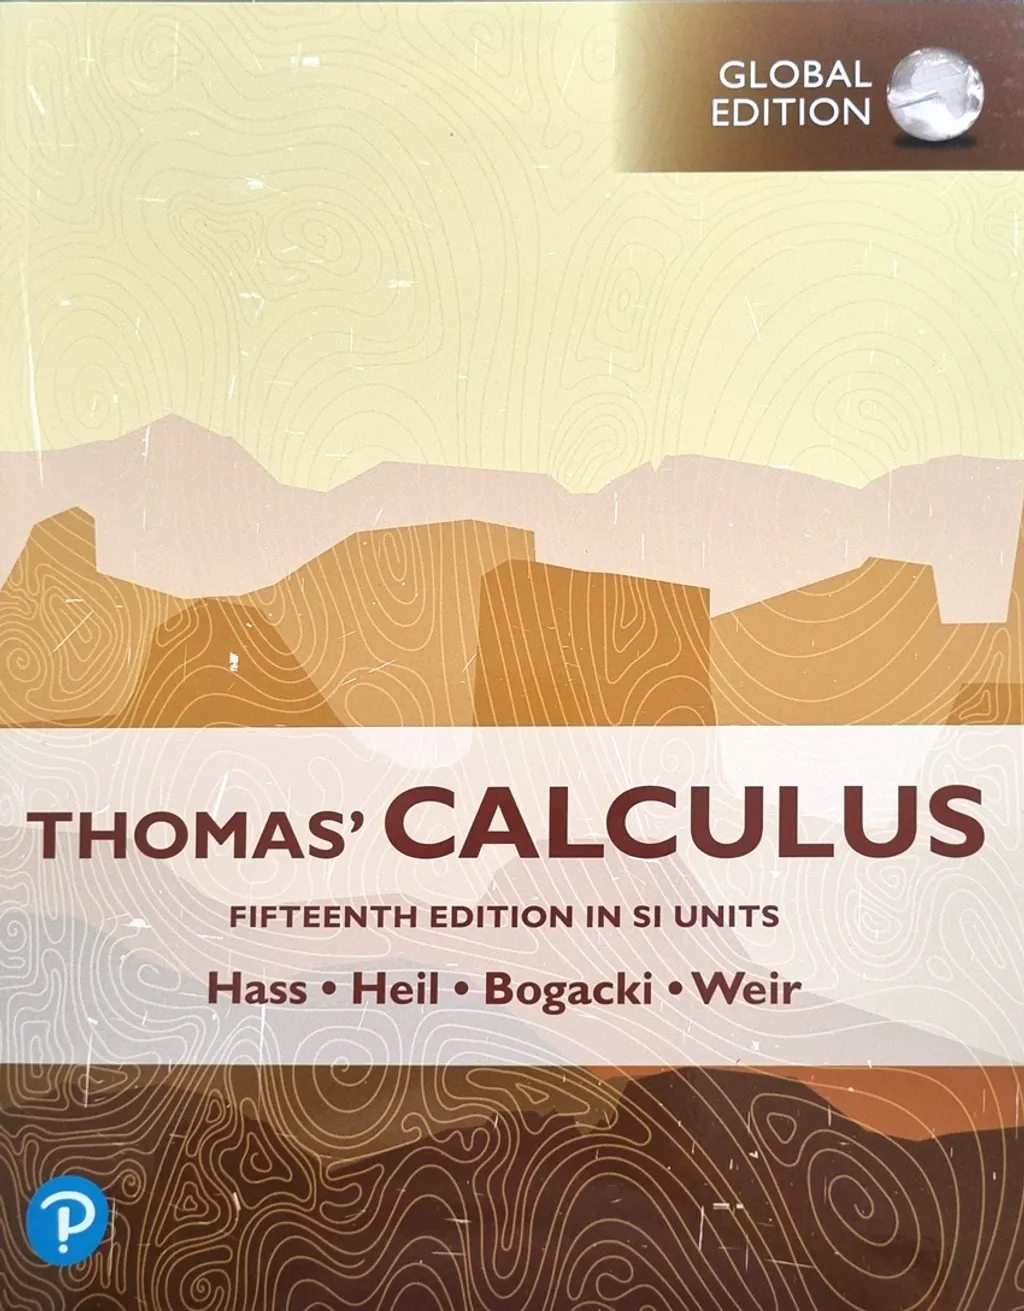
\includegraphics[scale=0.3]{./cover.png}
\end{center}

\subsection*{4.4 产品通路}
\addcontentsline{toc}{section}{4.4 产品通路}

由于托马斯微积分是一本备受欢迎的微积分教材,在全球拥有广泛消费群,且出版商Pearson Education没有实体门店,因此它的销售渠道主要是通过间接配销的方式,即通过全球各地书店、教育机构等渠道销售。

\subsection*{4.5 产品竞争对手}
\addcontentsline{toc}{section}{4.5 产品竞争对手}

托马斯微积分是一本备受欢迎的微积分教材,但市场上有其他一些竞争对手,提供类似的微积分教育资源。以下是一些与其竞争的微积分教材:

\begin{itemize}
    \item《Calculus》 by James Stewart

    \item 《Calculus》 by Michael Spivak

    \item 《A First Course in Calculus》 by Serge Lang

          \item《Calculus》 by Ron Larson and Bruce H. Edwards
\end{itemize}

\subsection*{4.6 产品推广}

\noindent\textbf{教材展示和教育会议}

\noindent 教材出版商通常会参加教育会议和展览,向教师和教育专业人士展示他们的微积分教材。这提供了一个机会,让教师了解教材的内容和教学方法。
~\\

\noindent\textbf{学校采购决策支持}

\noindent 教材出版商可能与学校、大学和学院的采购部门合作,以便将其微积分教材列入教育机构的采购清单。这种合作有助于确保教材在校园内广泛使用。
~\\

\noindent\textbf{教材配套资源}

\noindent 教材通常附带一系列在线学习资源、教学辅助材料和测试题库。出版商会积极推广这些资源,以增加教材的吸引力。
~\\

\noindent\textbf{教材样本}

\noindent 出版商提供免费或低成本的教材样本,供教师和教育机构评估。这有助于他们了解教材的内容和质量,以决定是否采用。
~\\

\section*{5. 参考文献}

\begin{enumerate}
    \item \url{https://rodrigopacios.github.io/mrpacios/download/Thomas_Calculus.pdf}
    \item \url{https://maa.org/press/maa-reviews/thomas-calculus}
    \item \url{https://en.wikipedia.org/wiki/Pearson_Education}
    \item \url{https://www.amazon.com/Thomas-Calculus-14th-Joel-Hass/dp/0134438981}
    \item \url{https://www.pearson.com/en-us/subject-catalog/p/thomas-calculus/P200000007103}
    \item \url{https://baike.baidu.com/item/%E6%89%98%E9%A9%AC%E6%96%AF%E5%BE%AE%E7%A7%AF%E5%88%86/10980457}
    \item \url{https://abakcus.com/best-calculus-books-for-self-study/}
    \item \url{https://singapore.kinokuniya.com/bw/9781292089799}
\end{enumerate}
\end{document}
